
\subsection{Evaluation Approach}

\subsubsection{Compressed Image Data From Canvas}
In the section \ref{sec:graphical-data-serialization-concept} the raw output from native Canvas is briefly described. The data exported by the method \textit{getImageData()} contains all values of each pixel without any compression. However, native Canvas also provides a method called \textit{toDataURL()}, which is able to export the image data with the specific image format. The default type is \textit{image/png}.

As a result, using \textit{toDataURL()} could achieve the compressed image  of a Canvas. Since the image format \textit{PNG} uses lossless compression, which combines the LZ77-based DEFLATE algorithm\footnote{https://en.wikipedia.org/wiki/DEFLATE - accessed 119 July 2016} with a selection of domain-specific prediction filters, \textit{PNG} format is chosen as the format of output image data  from Canvas for the evaluation\cite{barron1998minimum}. An example of the image data exported by calling \textit{toDataURL()} is shown in code listing \ref{list:toDataURL-eval}.


\begin{lstlisting}[language=JavaScript, caption=Example of image data while calling toDataURL() , label={list:toDataURL-eval}]
var canvas = document.getElementById("canvas");
var dataURL = canvas.toDataURL();
console.log(dataURL);
// "data:image/png;base64,iVBORw0KGgoAAAANSUhEUgAAAAUAAAAFCAYAAACNbybl...ADElEQVQImWNgoBMAAABpAAFEI8ARAAAAAElFTkSuQmCC"
\end{lstlisting}

\subsubsection{Measurement Process}
The serialized graphical data model adopted in Graphicuss system is presented in section \ref{sec:drawing-imp}. To evaluate the data space of each data model, the metric \textit{Byte} is taken for representing the length of data. In addition, two different dimensions are considered to evaluate the consumption of data space.

\begin{itemize}
  \item \textbf{Size of Canvas}: two different sizes \textit{800*600} and \textit{400*300} of Canvas are defined.
  \item \textbf{Amount of Components}: various amounts of components are drawn on the native Canvas and objectified Canvas in two different sizes.
\end{itemize}

The comparison is following the measurement process as below:

\begin{enumerate}
  \item Native Canvas or objectified Canvas with a certain size is initialized.
  \item 3 methods for drawing elements \textit{Rectangle}, \textit{Circle} and \textit{Line} in black color are predefined, which will be randomly chosen during the evaluation.
  \item Random components from the preset are selected to be drawn at a random position with a random scale on the Canvas.
  \item The length of the output data model is recorded for each amount of components in a range of 0 to 2000
\end{enumerate}

In general, four tests are performed for both types of Canvas in two different sizes. Figure \ref{fig:eval-size} illustrates the results of the test.


\begin{figure}[!htbp]
  \centering
    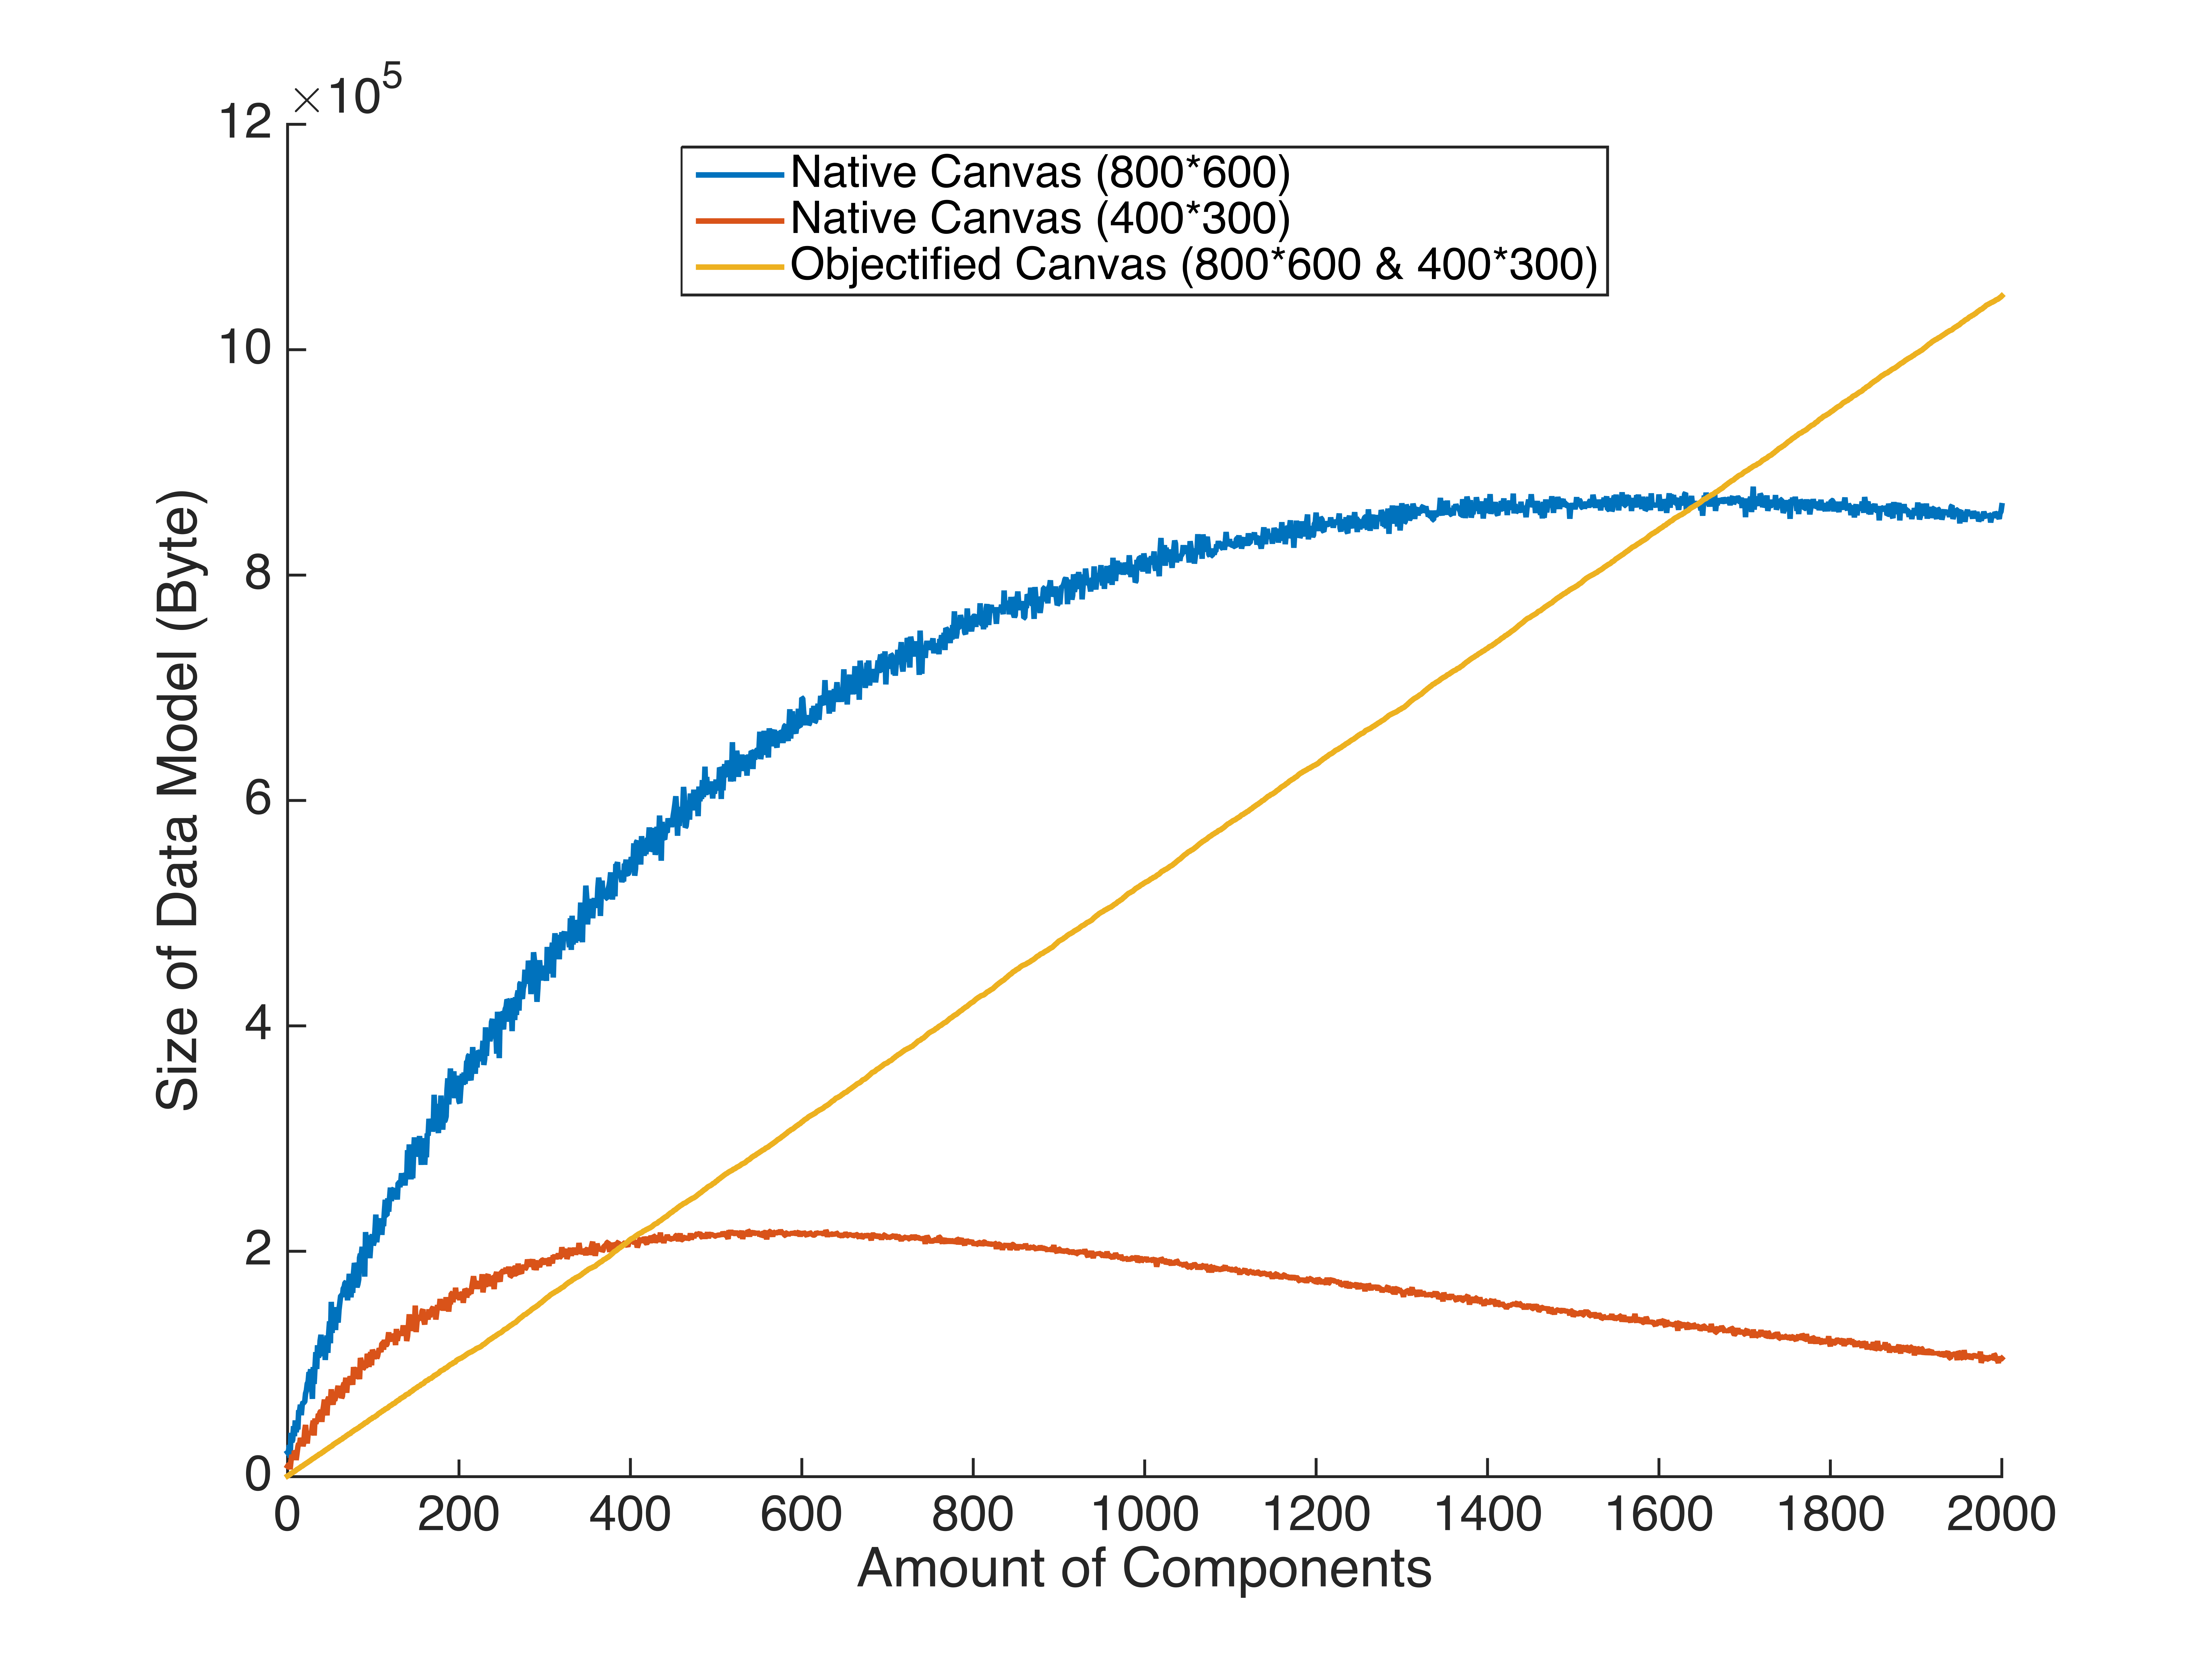
\includegraphics[width=1\textwidth]{Figures/eval-size.png}
  \caption{Comparison of data spaces of image data from native Canvas in two sizes(800*600, 400*300) and adopted graphical data model in Graphicuss}
  \label{fig:eval-size}
\end{figure}

\subsection{Analysis of Result }

Though four tests are executed, the figure \ref{fig:eval-size} shows only three curves or lines. The reason is that the results of objectified Canvas in two sizes are nearly same and overlap themselves on the figure. So the yellow line represents both results of objectified Canvas in  two sizes.

In overview, the data size correlates with the size of Canvas and amount of components drawn on Canvas. Therefore, both dimensions are analyzed separately in the following part.

\subsubsection{Dimension: Size of Canvas}


\textbf{Size of data model from objectified Canvas is irrelevant to the size of Canvas}. The yellow line on the figure shows both that results exported in different Canvas' size are generally same. Since the data model of objectified Canvas represents the components not pixels, the result is as expected.   

\textbf{Size of image data from native Canvas has a high-positive correlation with the size of Canvas}. As the output image data from native Canvas describes each pixel of the Canvas, size of the Canvas is one of the most important factors which affect the size of image data.

\textbf{Max size of image data from native Canvas is approximately linear to the size of Canvas}. The max size of image data from the blue curve is about $8\times 10^{5}$ Byte , while the max size from the orange curve is nearly $2\times 10^{5}$ Byte, which means, the former is 4 times as great as the latter. The size of \textit{800*600} is also 4 times greater than the size of \textit{400*300}, which also proves that the output image data describes each pixel.


\subsubsection{Dimension: Amount of Components}


\textbf{Size of data model from objectified Canvas is linear to the amount of components}. Because the data model from objectified Canvas is a composition of components' description, the data size increases linearly with the amount of components.

\textbf{Within a certain amount of components, the distribution of image data's size from native Canvas is logarithmic}. As the test shows, if less than about 1400 components are drawn on the native Canvas in size of 800*600, or less than 500 components in size of 400*300, the increment of data size is logarithmic due to the algorithm of image compression. With the increasing amount of components, the Canvas is getting more and more complex, the data size becomes greater as well.  

\textbf{Size of image data from native Canvas starts decreasing slightly after the amount of components reached its threshold}. Since all the randomly drawn components are all rendered in the single color black, almost all the pixels are in black if huge amount of components is drawn on the Canvas. Therefore, the complexity of the image is reduced. As a result, the compression of image data plays its role effectively and the size of image data decreases.

\textbf{In general, data model from objectified Canvas is much more efficient for storing than native Canvas}. As presented in the figure, if the amount of components is less than about 1650 components in size of 800*600, or less than 400 components in size of 400*300, the data model from objectified Canvas achieves much better efficiency in storing. When the amount of components reached the thresholds, then the native Canvas gains the upper hand. However, in the real world, normal users won't paint such a huge amount of components on a single Canvas.